% This program is free software: you can redistribute it and/or modify it under the te-
% ms of the GNU General Public License as published by the Free Software Foundation, e-
% ither version 3 of the License, or (at your option) any later version.
% 
% This program is distributed in the hope that it will be useful, but WITHOUT ANY WARR-
% ANTY without even the implied warranty of MERCHANTABILITY or FITNESS FOR A PARTICULAR
% PURPOSE. See the GNU General Public License for more details.
% 
% You should have received a copy of the GNU General Public License along with this pr- 
% ogram. If not, see https://www.gnu.org/licenses/. 


%! ~~~ Packages Setup ~~~ 
\documentclass[]{article}
\usepackage{lipsum}
\usepackage[paper=portrait,pagesize]{typearea}


% Math packages
\usepackage[usenames]{color}
\usepackage{forest}
\usepackage{ifxetex,ifluatex,amssymb,amsmath,mathrsfs,amsthm,witharrows,mathtools,mathdots}
\usepackage{amsmath}
\WithArrowsOptions{displaystyle}
\renewcommand{\qedsymbol}{$\blacksquare$} % end proofs with \blacksquare. Overwrites the defualts. 
\usepackage{cancel,bm}
\usepackage[thinc]{esdiff}


% tikz
\usepackage{tikz}
\usetikzlibrary{graphs}
\newcommand\sqw{1}
\newcommand\squ[4][1]{\fill[#4] (#2*\sqw,#3*\sqw) rectangle +(#1*\sqw,#1*\sqw);}


% code 
\usepackage{algorithm2e}

% Design
\usepackage[labelfont=bf]{caption}
\usepackage[margin=0.1in]{geometry}
\usepackage{wrapfig,multicol}
\usepackage[skip=2pt, indent=0pt]{parskip}
\usepackage[normalem]{ulem}
\forestset{default}

\usepackage{titlesec}
	\definecolor{secblue}{RGB}{0, 50, 180}
	\titleformat{\section}[block]
		{\fontsize{11}{11}}
		{\regFont (\thesubsection) \!\!\dotfill}
		{0em}
		{\color{secblue}\fontsize{7}{6}\rmfamily\bfseries}
	
	\definecolor{subsecblue}{RGB}{10, 100, 180}
	\titleformat{\subsection}[block]
		{\fontsize{11}{11}}
		{\regFont(\thesubsection) \hfill}
		{0.5em}
		{\bf\color{subsecblue}\regFont\bfseries}
\usepackage{graphicx}
\graphicspath{ {./} }

\usepackage[colorlinks]{hyperref}
\usepackage{hyperref}
\hypersetup{pdftitle={SCS by Shahar Perets}}

%\BeforeBeginEnvironment{alignat*}{\vspace{-17pt}}
%\AfterEndEnvironment{alignat*}{\vspace{-19pt}}
\BeforeBeginEnvironment{alignat}{\vspace{-17pt}}
\AfterEndEnvironment{alignat}{\vspace{-27pt}}
\BeforeBeginEnvironment{forest}{\vspace{-12pt}}
\AfterEndEnvironment{forest}{\vspace{-7pt}}
\BeforeBeginEnvironment{algorithm}{\vspace{-5pt}}
\AfterEndEnvironment{algorithm}{\vspace{-5pt}}

\newcommand\compactsubsection[1]        {\vspace{-10pt}\subsection{#1}\vspace{-6pt}}
\newcommand\compactsection   [1]        {\vspace{-10pt}\section{#1}\vspace{-6pt}}
\newcommand\subsectionrightaftersection {\vspace{10pt}}

\theoremstyle{definition}
\definecolor{theoColor}{RGB}{10, 100, 30}
\newtheorem{Theorem}{\color{theoColor}Theorm}
\definecolor{defiColor}{RGB}{100, 30, 10}
\newtheorem{Definition}{\color{defiColor}Definition}
\definecolor{lemColor}{RGB}{90, 90, 10}
\newtheorem{Lemma}{\color{lemColor}Lemma}
\newtheorem{Remark}{\textit{Remark}}


\newcommand\theo  [1] {\begin{Theorem}#1\end{Theorem}}
\newcommand\defi  [1] {\begin{Definition}#1\end{Definition}}
\newcommand\rmark [1] {\begin{Remark}#1\end{Remark}}
\newcommand\lem   [1] {\begin{Lemma}#1\end{Lemma}}

%! ~~~ Math shortcuts ~~~

% Letters shortcuts
\newcommand\N     {\mathbb{N}}
\newcommand\Z     {\mathbb{Z}}
\newcommand\R     {\mathbb{R}}
\newcommand\Q     {\mathbb{Q}}
\newcommand\C     {\mathbb{C}}
\newcommand\E     {\mathbb{E}}

\newcommand\powerset {\mathcal{P}}
\newcommand\oc    {\mathcal{O}}
\newcommand\zc    {\mathcal{Z}}

\newcommand\Si    {\Sigma}

\newcommand\epsi  {\epsilon}
\newcommand\vepsi {\varepsilon}
\newcommand\vphi  {\varphi}

\newcommand\other {\mathrm{else}}
\newcommand\set   {\ell et \text{ }}

\newcommand\ra    {\rangle}
\newcommand\la    {\langle}

\newcommand\rc    {\right\rceil}
\newcommand\lc    {\left\lceil}
\newcommand\rf    {\right\rfloor}
\newcommand\lf    {\left\lfloor}
\newcommand\ceil  [1] {\lc #1 \rc}
\newcommand\floor [1] {\lf #1 \rf}

\newcommand\seq   {\overset{!}{=}}
\newcommand\slh   {\overset{LH}{=}}
\newcommand\sle   {\overset{!}{\le}}
\newcommand\sge   {\overset{!}{\ge}}
\newcommand\sll   {\overset{!}{<}}
\newcommand\sgg   {\overset{!}{>}}

\newcommand\ol    {\overline}

\newcommand\ta    {\theta}
\newcommand\ap    {\alpha}

\renewcommand\inf {\infty}
\newcommand  \ninf{-\inf}

\newcommand\sumnk     {\sum_{k = 0}^{n}}
\newcommand\sumni     {\sum_{i = 0}^{n}}
\newcommand\sumnio    {\sum_{i = 1}^{n}}
\newcommand\sumai     {\sum_{i = 1}^{n} A_i}
\newcommand\co        {\colon}


% Greek Letters
\newcommand\ag        {\alpha}
\newcommand\bg        {\beta}
\newcommand\cg        {\gamma}
\newcommand\dg        {\delta}
\newcommand\eg        {\epsi}
\newcommand\zg        {\zeta}
\newcommand\hg        {\eta}
\newcommand\tg        {\theta}
\newcommand\ig        {\iota}
\newcommand\kg        {\keppa}
\renewcommand\lg      {\lambda}
\newcommand\og        {\omicron}
\newcommand\rg        {\rho}
\newcommand\sg        {\sigma}
\newcommand\yg        {\usilon}
\newcommand\wg        {\omega}

\newcommand\Dg        {\Delta}
\newcommand\Wg        {\Omega}

\newcommand\logn      {\log n}

% Other shortcuts
\newcommand\op    {^{-1}}

\newcommand\sof[1]    {\left | #1 \right |}
\newcommand\cl [1]    {\left ( #1 \right )}
\newcommand\csb[1]    {\left [ #1 \right ]}
\newcommand\ccb[1]    {\left \{ #1 \right \}}

\newcommand\bs        {\blacksquare}
\newcommand\dequad    {\!\!\!\!\!\!}
\newcommand\dequadd   {\dequad\duquad}

% DS
\newcommand\limsi     {\limsup_{n \to \inf}}
\newcommand\limfi     {\liminf_{n \to \inf}}

\DeclareMathOperator\amort   {amort}
\DeclareMathOperator\worst   {worst}
\DeclareMathOperator\type    {type}
\DeclareMathOperator\cost    {cost}
\DeclareMathOperator\tim     {time}

\definecolor{codeblue}{rgb}{0,0,0.5}
\definecolor{codegreen}{rgb}{0,0.35,0}
\newcommand\importDs{
	\SetKwProg{Fn}{function}{ is}{end}
	\SetKwData{error}{\color{codered}error}
	\SetKwInOut{Input}{input}
	\SetKwInOut{Output}{output}
	\SetKwRepeat{Do}{do}{while}
	\SetKwData{Null}{\color{codegreen}null}
	\SetKwData{True}{\color{codeblue}true}
	\SetKwData{False}{\color{codeblue}false}
}


% Algorithms
\newcommand\sFunc [1] {\SetKwFunction{#1}{#1}}
\newcommand\sData [1] {\SetKwData{#1}{#1}}
\newcommand\sIO   [1] {\SetKwInOut{#1}{#1}}
\newcommand\io    [2] {\Input{#1}\Output{#2}\BlankLine}

%! ~~~ Document ~~~

\newcommand\regFont   {\fontsize{5}{6}\rmfamily}
\newcommand\tableFont {\fontsize{5}{4}\rmfamily}
\DeclareMathOperator  {\midText}{mid}
\newcommand\tline[2]  {$\overset{\text{#1}}{\text{#2}}$}

\author{Shahar Perets}
\title{Shit Cheat Sheet $\sim$ Data Structures $\sim$ \textit{2025B}}
\begin{document}
%	\setlength{\columnseprule}{0.2pt}
	\setlength{\intextsep}{0pt}
	\setlength{\columnsep}{4pt}
	\KOMAoptions{paper=landscape,pagesize}
	\recalctypearea
	\areaset{2.42\textwidth}{2.24\textheight}
	\regFont
	
	\begin{multicols}{4}
%		{\hfil \fontsize{12}{11}\rmfamily Shahar Perets $\sim$ Shit Cheat Sheet}
		\regFont
%		\vspace{-3pt}
		\compactsection{ADTs}
			\textbf{List. }\texttt{List()}, \texttt{Retrieve($L, i$)}, \texttt{Insert($L, b, i$)}, \texttt{Delete($L, i$)}, \texttt{Length($L$)} \textit{optional:} \texttt{Search($L, b$)}, \texttt{Concat($L_1, L_2$)}, \texttt{Plant($L_1, i, L_2$)}, \texttt{Split($L, i$)} \textit{special cases:} \texttt{Retrieve/Insert/Delete-First/Last}. 
			
			\textbf{Dictionary. }\texttt{Dictionary()}, \texttt{Insert($D, x$)}, \texttt{Delete($D, x$)}, \texttt{Search($D, k$)}, \texttt{Min($D$)}, \texttt{Max($D$)}, \texttt{Successor($D, x$)}, \texttt{Predecessor($D, x$)} \textit{(for rank trees): }\texttt{Select($D, k$)} [the k$^{\text{th}}$ smallest element], \texttt{Rank($D, x$)} [the position in sorted order]. 
			
			\textbf{Stack. }(LIFO) \texttt{Push($L, b$)} [=ins.-last], \texttt{Top($L$)} [=ret.-last], \texttt{Pop($L$)} [=del.-last]. (all $\oc(1)$ using arrays)
			
			\textbf{Queue. }(FIFO) \texttt{Enqueue($L, b$)} [=ins-last], \texttt{Head($L$)} [=ret.-first], \texttt{Dequeue($L$)} [=del-first]. (all $\oc(1)$ using circular arrays)
			
			\textbf{Deque. }Queue + Stack
			
			\textbf{Priority Queue. }\texttt{Insert($x, Q$)}, \texttt{Min($Q$)}, \texttt{Delete-Min($Q$)}, (optional:) \texttt{Decrease-Key($x, Q, \Delta$)}, \texttt{Delete($x, Q$)}
			
			\textbf{Vector. }\texttt{Vector($m$)}, \texttt{Get($V, i$)}, \texttt{Set($V, i, \mathrm{val}$)}. (All $\oc(1)$ using \textit{legals} and \textit{positions} arrays that reference each other)
			
			\begin{algorithm}[H]\importDs\sData{positions}\sData{legals}\sFunc{isGarbage}
				\Fn{\isGarbage{$i$}}{
					\If{$0 \le \positions[i] < \legals.size$ {\bf and} $\legals[\positions[i]] = i$}{
						\Return{\False}
					} \Return{\True}
				}
			\end{algorithm}
			
			\textbf{Graph. }\texttt{Edge($i, j$)}, \texttt{Add-Edge($i, j$)}, \texttt{Remove-Edge($i, j$)}, \texttt{InDeg($i$)}, \texttt{OutDeg($i$)} etc.
			
			\vspace{-3pt}
			\compactsection{Graphs}
			\vspace{-1pt}
			\begin{Definition}[Topological sorting algo.]
				Input: directed graph / Output: numbering $(n_i)_{i = 1}^{N}$ of the graph nodes where $\forall (i, j) \in E \co n_i < n_j$. 
			\end{Definition}
			\theo{Topological Sorting exists iff the graph doesn't contain cycles.}
			\begin{algorithm}[H]
				\importDs\sData{k}\sData{v}
				\k $\gets$ $0$\;
				\While{there are sources}{
					find source \v\;
					$n_i \gets k$\; $k \gets k + 1$\;
					remove $v$ from the graph
				}
				if $\k = n$ numbering completed, otherwise isn't possible. 
			\end{algorithm}
			building ``source queue'' takes $\oc(n)$, dequeuing source $\oc(1)$, and enqueuing new sources to sources-queue $\oc(d_{\mathrm{out}}(i))$. Total $\oc(n + m)$ for topological ordering. 
			\begin{Definition}[source]
				is a node that has no incoming edges. 
			\end{Definition}
			\begin{Remark}
				any DAG has at least one source
			\end{Remark}
			
		\vspace{-4pt}
		\compactsection{Complexity}
			\vspace{-1pt}
			\begin{Definition}
				Suppose there's a data structure with $k$ types of operations $(T_i)_{i = 1}^{k}$, then for sequence of operations $(op)_{i = 1}^{n}$, then:
				
				\hfil $\mathrm{time}(op_1 \dots op_n) \le \sumni \mathrm{bound}(\type(op_i))$
				
				Where (W.C. bound) $\worst(T_i)$ is the maximal time for a single operation typed $T_i$, and (amortized bound) $\amort(T_i)$ is a series of bounds for cost of every valid sequence $(op_i)_{i = 1}^{n}$. 
				
				\textbf{Amortization methods. }aggregation (regular average), accounting (bank method), and potential function (defined to be the balance of the bank) that satisfies $\amort(op_i) = \mathrm{time}(op_i) + \Phi_i - \Phi_{i - 1}$. 
			\end{Definition}
			\vspace{-14pt}\begin{alignat*}{9}
				&\textstyle\sum_{i = 0}^{n} x^i          &&= \tfrac{x^{n + 1} - 1}{x - 1} = \Theta(x^n)  \quad\quad(x \neq 1) \\
				&\textstyle\sum_{i = 1}^{n} \tfrac{1}{i} &&= H_n = \Theta(\logn) \\
				&\textstyle\log n!                       &&= \Theta(n\logn) \\
				&\textstyle \ag + \bg = 1 \land          &&T(n) \le cn + T(\ag) + T(\bg n) \implies T(n) = \oc(n) \\
				&\textstyle \forall \ag < 1 \co          &&T(n) = T(\floor{\ag n}) + T(\floor{(1 - \ag)n}) + 1 = \oc(n)
			\end{alignat*}\vspace{-10pt}
			
			\vspace{-4pt}
			\compactsubsection{Asymptotic Notations}
			\vspace{-5pt}
			\begin{alignat*}{9}
				f &= O(g) &&\iff \exists n_0, c > 0\, \forall n \ge n_0\co f(n) \le c g(n) \\
				f &= \Omega(g) &&\iff \exists n_0, c > 0\, \forall n \ge n_0\co f(n) \ge c g(n) \\
				f &= \Theta(g) &&\iff f = \Omega(g) \land f = O(g) \\
				f &= o(g) &&\iff \forall c\, \exists n_0\, \forall n \ge n_0\co f(n) \le cg(n) \\
				f &= \omega(g) &&\iff \forall c\, \exists n_0\, \forall n \ge n_0\co f(n) \ge cg(n)
			\end{alignat*}
			\vspace{-15pt}
			\begin{gather*}
				f = \Omega(g) \iff g = O(f) \\
				\dequad f_1 = O(g_1) \land f_2 = O(g_2)\quad\quad\quad\quad  \\ \quad\quad\quad\quad  \implies f_1(n) + f_2(n) = O(\max(g_1(n), g_2(n)))
			\end{gather*}
			\vspace{-15pt}
			\begin{alignat*}{9}
				f &= O(g)      &&\iff \limsup_{n \to \inf} \textstyle \frac{f(n)}{g(n)} &&< \inf \\
				f &= \Omega(g) &&\iff \limsup_{n \to \inf} \textstyle \frac{f(n)}{g(n)} &&> 0 \\
				f &= o(g)      &&\iff \lim_{n \to \inf}    \textstyle \frac{f(n)}{g(n)} &&= 0 \\
				f &= \omega(g) &&\iff \lim_{n \to \inf}    \textstyle \frac{f(n)}{g(n)} &&= \inf
			\end{alignat*}
			
			\compactsubsection{Master Theorem}
				let $ f \colon \R \to \R $ be an function, and let $ a \ge 1, b > 1 $ be constants, assuming $ T \colon \R_{\ge 0} \to \R, \ T(n) = a \cdot T\left (\tfrac{n}{b} \right ) + f(n)$, then: 
				\begin{enumerate}
					\item $ \exists \vepsi > 0. f(n) = O(n^{\log_b a - \vepsi}) $ \\ $\implies T(n) = \Theta(n^{log_b a}) $
					\item $ f(n) = \Theta(n^{\log_b a}) $ \\ $\implies T(n) = \Theta(n^{log_b a} \cdot \logn) $
					\item $ \exists \vepsi > 0. f(n) = \Omega(n^{\log_b a + \vepsi}) \land $ \\
					$\ \exists c < 1, n_0 \ge 0. \forall n \ge n_0. a \cdot f(\tfrac{n}{b}) \le c \cdot f(n) $ \\
					$\implies T(n) = \Theta(f(n)) $
				\end{enumerate}
				\textit{Note that $ \mathit{\tfrac{n}{b}} $ could be $ \mathit{\lf \tfrac{n}{b} \rf} $ nor $ \mathit{\lc \tfrac{n}{b} \rc} $}
		
		\vspace{-3pt}				
		\compactsection{Dictionaries}\subsectionrightaftersection
			\compactsubsection{General Trees}
				\begin{Definition}[full tree]
					all internal nodes have exactly $i$ children. 
				\end{Definition}
				\begin{Definition}[BST]
					satisfies: $\forall x \forall y$ if $y$ is in the left subtree of $x$, then $y.key < x.key$, and vise-versa. 
				\end{Definition}
				\begin{Definition}[Node's Height]
					is the maximal length of downward path between that node and a leaf. 
				\end{Definition}
				\begin{Definition}[Node's Depth]
					is the length of the path up the tree to the root. 
				\end{Definition}
				\theo{minimal height of a tree is $\floor{\log n}$}
				\begin{Definition}[Balanced BST]
					if $h = \oc(\logn)$. 
				\end{Definition}
				\theo{for a given set of $n$ distinct keys, there are $\frac{1}{n + 1}\binom{2n}{n}$ (catalan number) BSTs. }
				\theo{the expected search complexity in a random BST is $\le (1 + 4 \logn)$. }
				\lem{the heights of a binary tree containing $\ell$ leaves $\ge \log \ell$. }
				
				\textbf{Tree walks. }pre: head $\to$ SLR, in: LSR, post: LRS
				
				
			\compactsubsection{AVL trees}
				\defi{$\mathrm{BF}(v) = h(v.\mathrm{left}) - h(v.\mathrm{right})$}
				\begin{Definition}[AVL Tree]
					a BST where $\forall v \in V \co \sof{\mathrm{BF}(v)} \le 1$
				\end{Definition}
				\theo{an AVL tree is balanced. Further more: $h \le \log_{\Phi}n \approx 1.44\logn$. }
				
				\begin{wrapfigure}{r}{0.6\linewidth}
					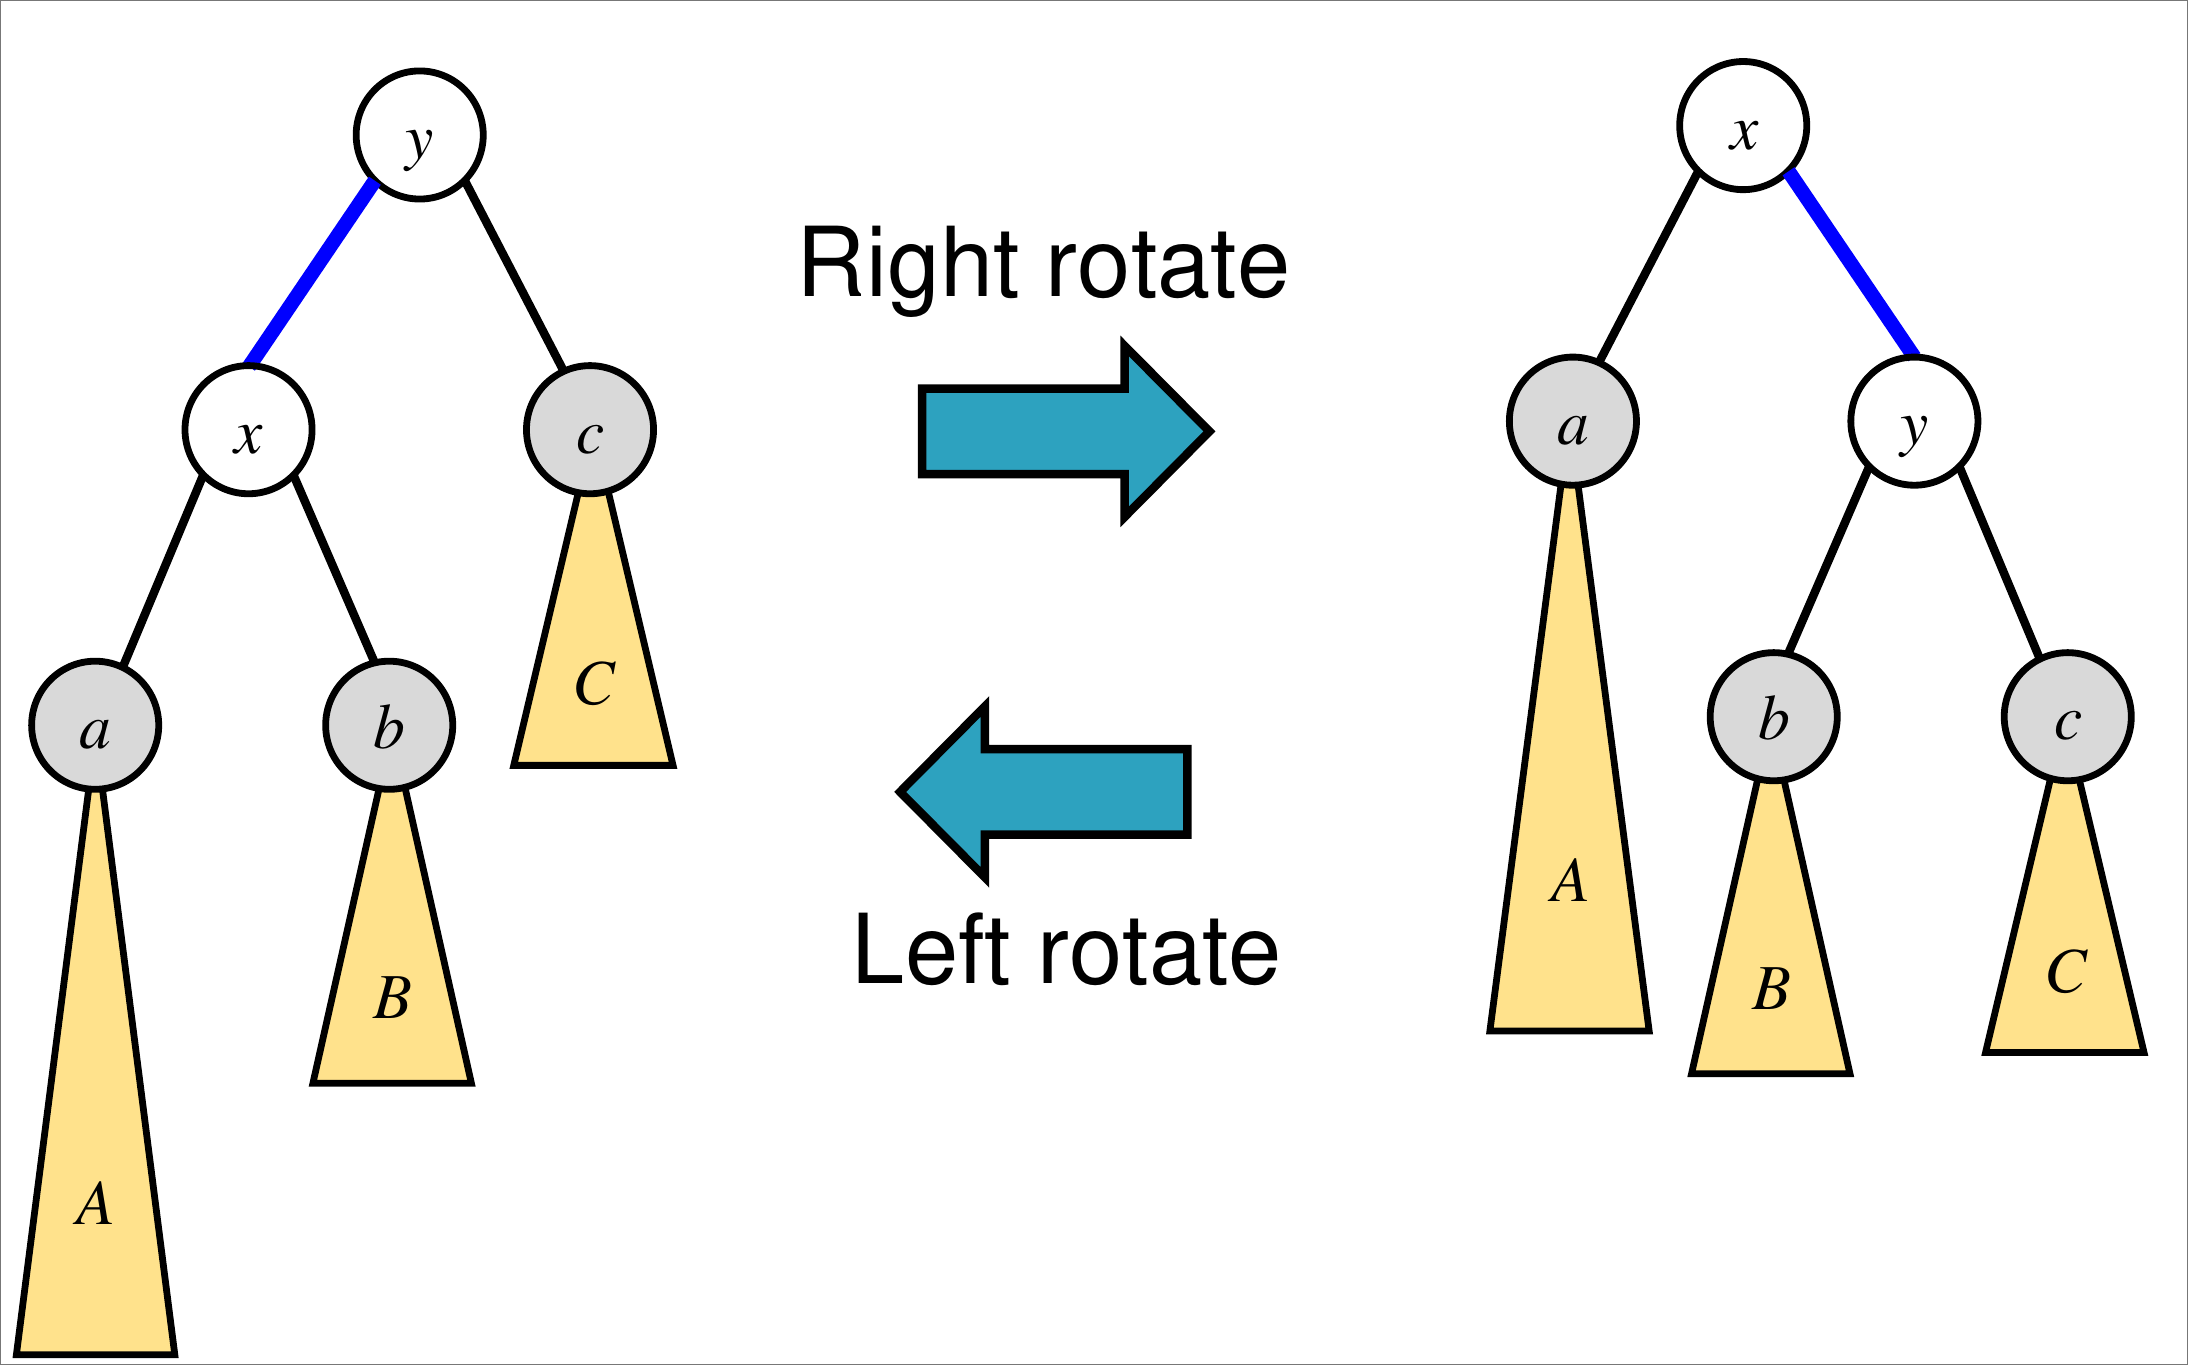
\includegraphics[width=\linewidth]{images/rotations}
					\vspace{-20pt}
				\end{wrapfigure}
				\textbf{Rotations. }see image
				\begin{Definition}[Fibonacci Tree]
					$F_i$ is: \\ \vspace{3pt} \begin{center}
						\begin{forest}
							[$F_i$ [$F_{i -1}$] [$F_{i - 2}$]]
						\end{forest}
					\end{center}
				\end{Definition}\vspace{2pt}
				\theo{an AVL tree with minimum edges is a fibonacci tree, has a size of $f_{h + 3} - 1$. }
				\begin{Definition}[Rank Tree]
					a tree that maintains the size of each subtree, hence supports the rank \& select operations in $\oc(\logn)$. 
				\end{Definition}
				\textbf{Example. }see image (nvm the colors)
				\begin{wrapfigure}{r}{0.6\linewidth}
					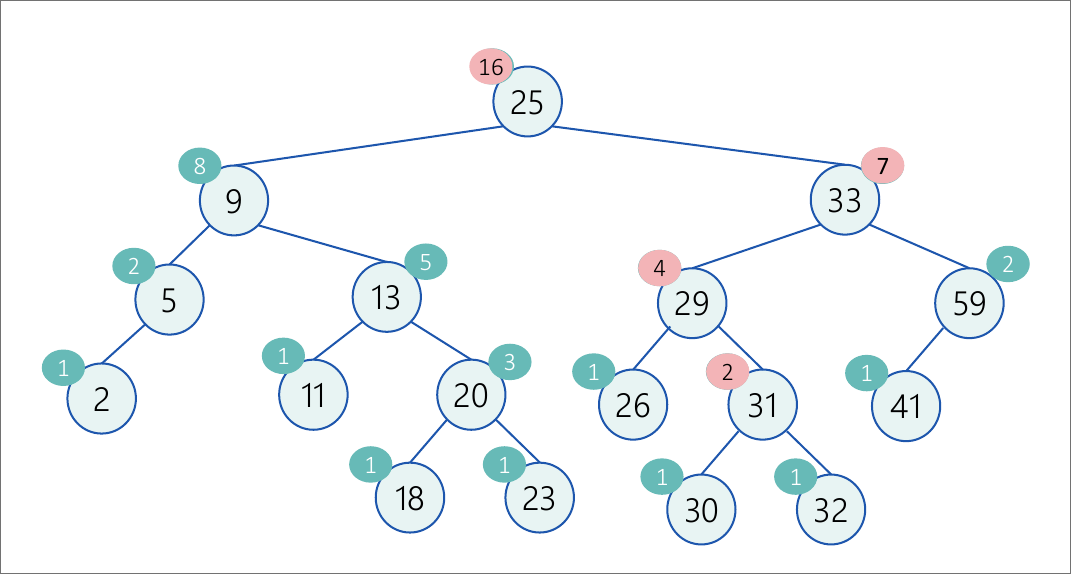
\includegraphics[width=\linewidth]{images/rankTreeExample}
				\end{wrapfigure}
				\textbf{\texttt{Tree-Select($T, k$)}: }start with $x \gets T.\mathrm{root}$, then let $r \gets x.\mathrm{left}.\mathrm{size} + 1$, if $k = r$ halt, otherwise if $k < r$ return \texttt{Select($x.\mathrm{left}, k$)} and if $k > r$ return \texttt{Select($x.\mathrm{right}, k - r$)}. 
				\theo{if the information that a given attribute $f$ defined for each node, can be computed merely from its direct children (\color{defiColor}local attribute\color{black}), then we can maintain $f$ in an AVL tree. }
				\begin{Remark}
					The theorem above is sufficient condition but not necessary. 
				\end{Remark}
				\,\!\vspace{-1em}
				\begin{wrapfigure}{l}{0.4\linewidth}
					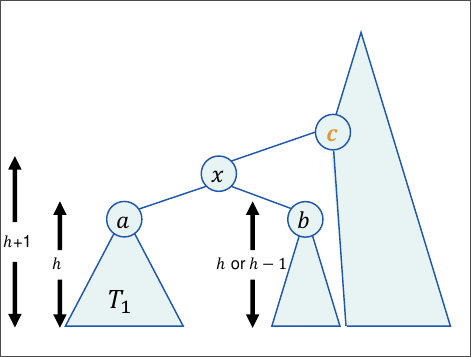
\includegraphics[width=\linewidth]{images/join2}
%					\vspace{1em}
				\end{wrapfigure}
				
				\vspace{-2em}
				\textbf{\texttt{Join($T_1, T_2$): }} where $T_1 < x < T_2$ is done $\oc(h_{T_1} + h_{T_2} + 1)$ (see image). \\
				\textbf{\texttt{Split($T, x$)}: }splits $T$ into $T_1 < x < T_2$ in $\oc(\logn)$ using joins (image next column). 
				
				\lem{the sum of the keys lesser than $v$, and the sum of the keys in the subtrees, can be implemented both without harming time complexity. }
				\lem{\texttt{Between}($s, t$) $=$ \texttt{Tree-Rank}($t$) $-$ \texttt{Tree-Rank}($s$) $+$ $1$}
				
				\begin{Definition}[Finger Tree]
					a tree that has a pointer to a specific node. 
				\end{Definition}
				\textbf{Split (yellow $< x < $ red):}
				
				\,\!\vspace{-3em}
				\begin{wrapfigure}{r}{0.2\linewidth}
					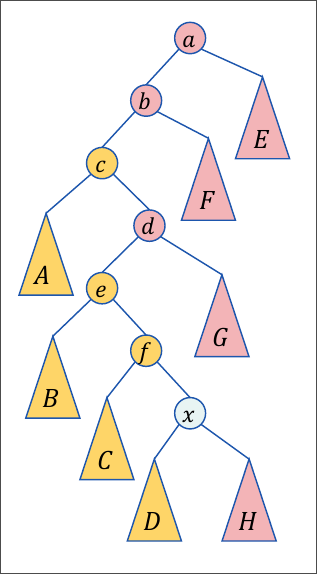
\includegraphics[width=\linewidth]{images/split}\vspace{-1em}
				\end{wrapfigure}
				\theo{in a finger tree \texttt{Select($T, k$)} can be implemented in $\oc(\log k)$. }
				\theo{Given a sorted array, we can create an AVL tree in $\oc(n)$ on which $h = \floor{\logn}$}
				

				\textbf{Insertion Fix: }if $\sof{\mathrm{BF}} = 2$ rotate and terminate, if $|\mathrm{BF}| < 2$ and height hasn't change, terminate, otherwise recursively preform this fix for the parent. (the zero case in blue at the above image doesn't matter for insertions) \\
				\textbf{Deletion Fix: }same as insertions, but with the case for son's $\mathrm{BF}=0$, and without terminating after rotation (since rotation may not restore the height of the subtree prior the insertion). \\
				\textbf{Amort. Bounds: }in any sequence of insertions only/deletions only, the amoritzed cost of rebalncing if $\oc(1)$ for $\Phi = \# \text{balanced nodes}$ or 1\$ on each balanced node. \\
				\textbf{Insertion Sort to AVL with Max. pointer: }has a complexity of $\oc\cl{n \log\cl{\frac{I}{n} + 2}}$ (see more info under 6.1)
%				\textbf{Regular Insertion Sort: }$\oc(n + I)$. 
				\begin{center}
					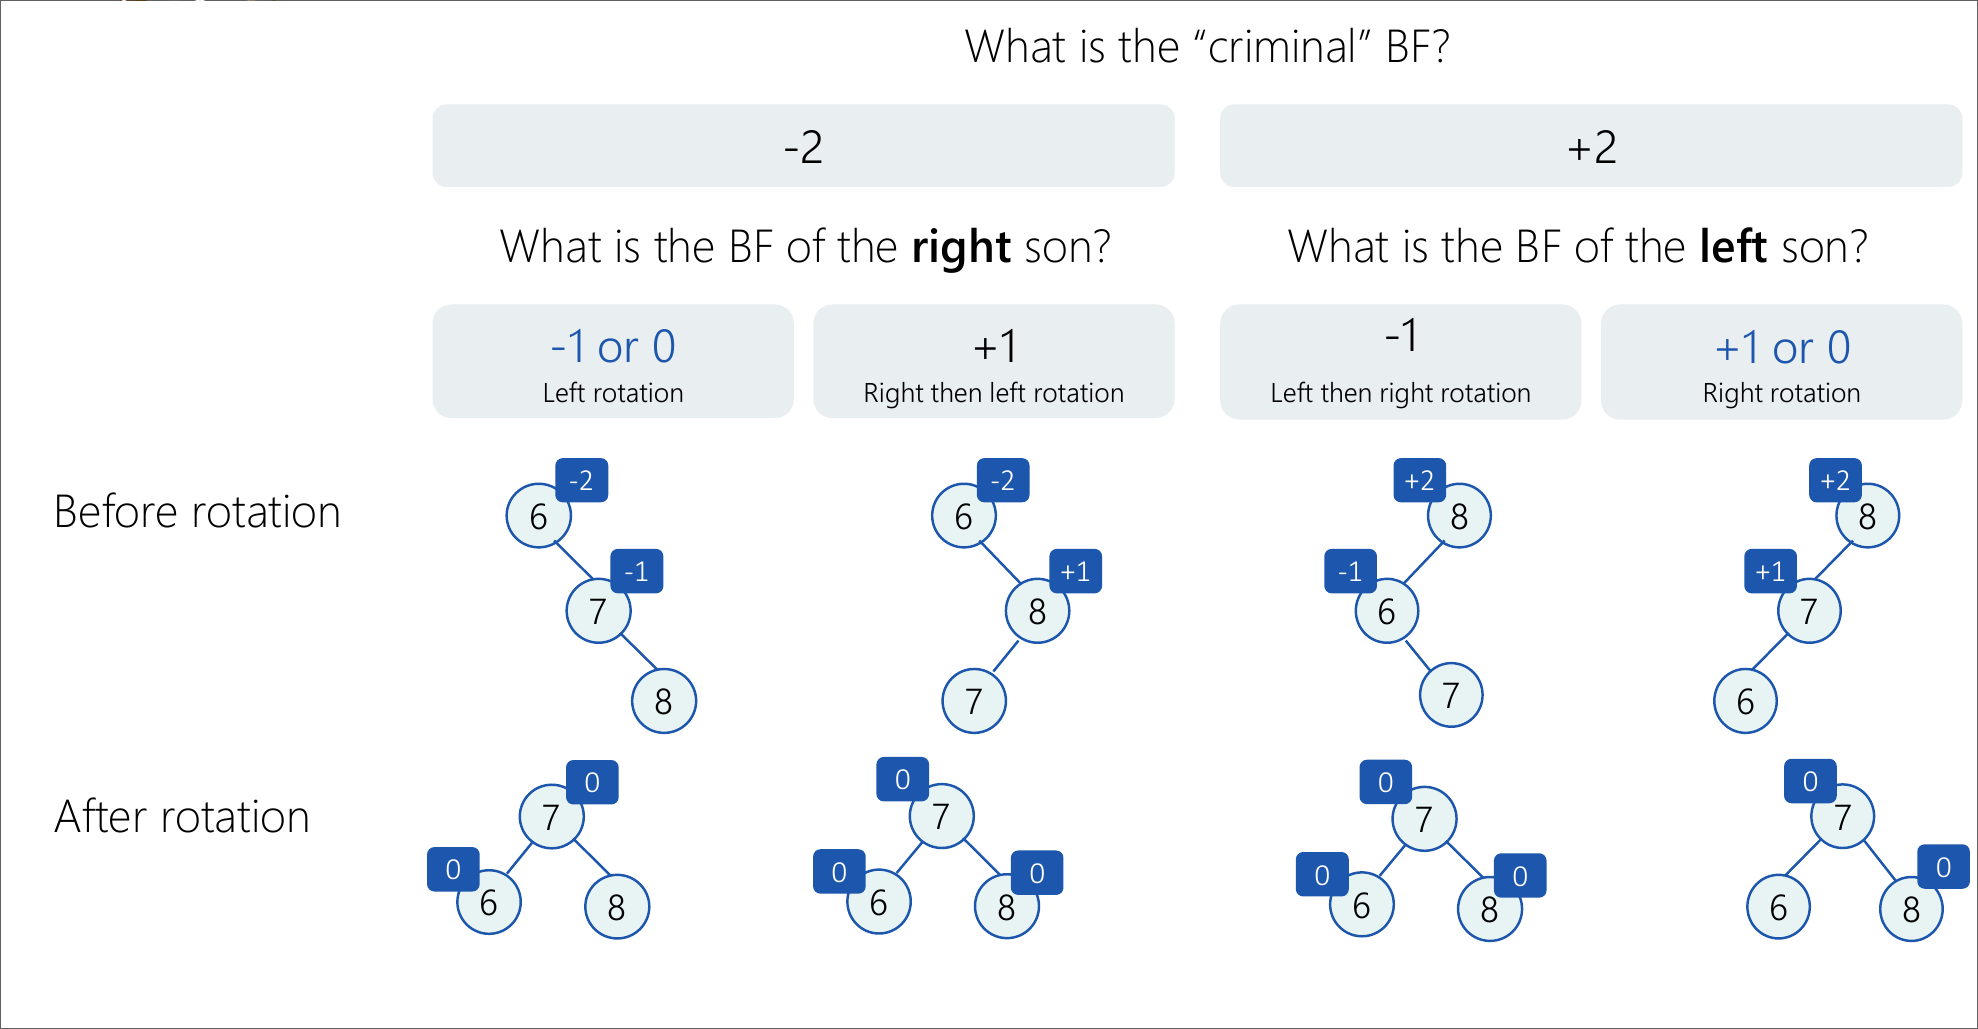
\includegraphics[width=0.75\linewidth]{images/rotationTableDeletion}
				\end{center}
			
			\vspace{-5pt}
			\compactsubsection{B-trees}		
				\begin{Definition}[B-tree]
					B-tree $(d, 2d)$ satisfies: 
					\begin{enumerate}
						\item each non-leaf expect for the root has $d \le r \le 2d$ children (hence $d - 1$ to $2d - 1$ keys);
						\item all leaves are at the same depth;
						\item the root has between $2$ and $2d$ children (hence $1$ to $2d - 1$ keys). 
					\end{enumerate}
				\end{Definition}
				\begin{Definition}[B$^{\text{+}}$-tree]
					a B-tree with keys only on leafs. 
				\end{Definition}
				\begin{Definition}[B$^{\text{*}}$-tree]
					B-tree with nodes $\frac{2}{3}$ full (instead of $\frac{d}{2d} = \frac{1}{2}$ full). 
				\end{Definition}
				\theo{at depth $h$ there are at least $2d^{h - 1}$ nodes. }
				\theo{a B-tree $(d, 2d)$ with $n$ edges and $h$ height fulfills $n \ge d^{h}$, $h \le \log_{d} n$}
				\theo{search in a b-tree requires $\oc(\log_dn)$ I/Os, and $\oc(\log_2 d \cdot \log_d n) = \oc(\logn)$ operations in total. }
				\lem{In a B-tree $\# \text{leaves} = \# \text{internal nodes} + 1$}
				
				\theo{Ins./Del. rebalancing cost is W.C. $\oc(\logn)$, and using button-up amort. (ins.+del.) $\oc(1)$, using top-down $\Omega(\log_dn)$}
				\textbf{Fuse} see right; \textbf{Split} see left; \textbf{Borrow} see bottom \\
				\vspace{-8pt}\begin{center}
					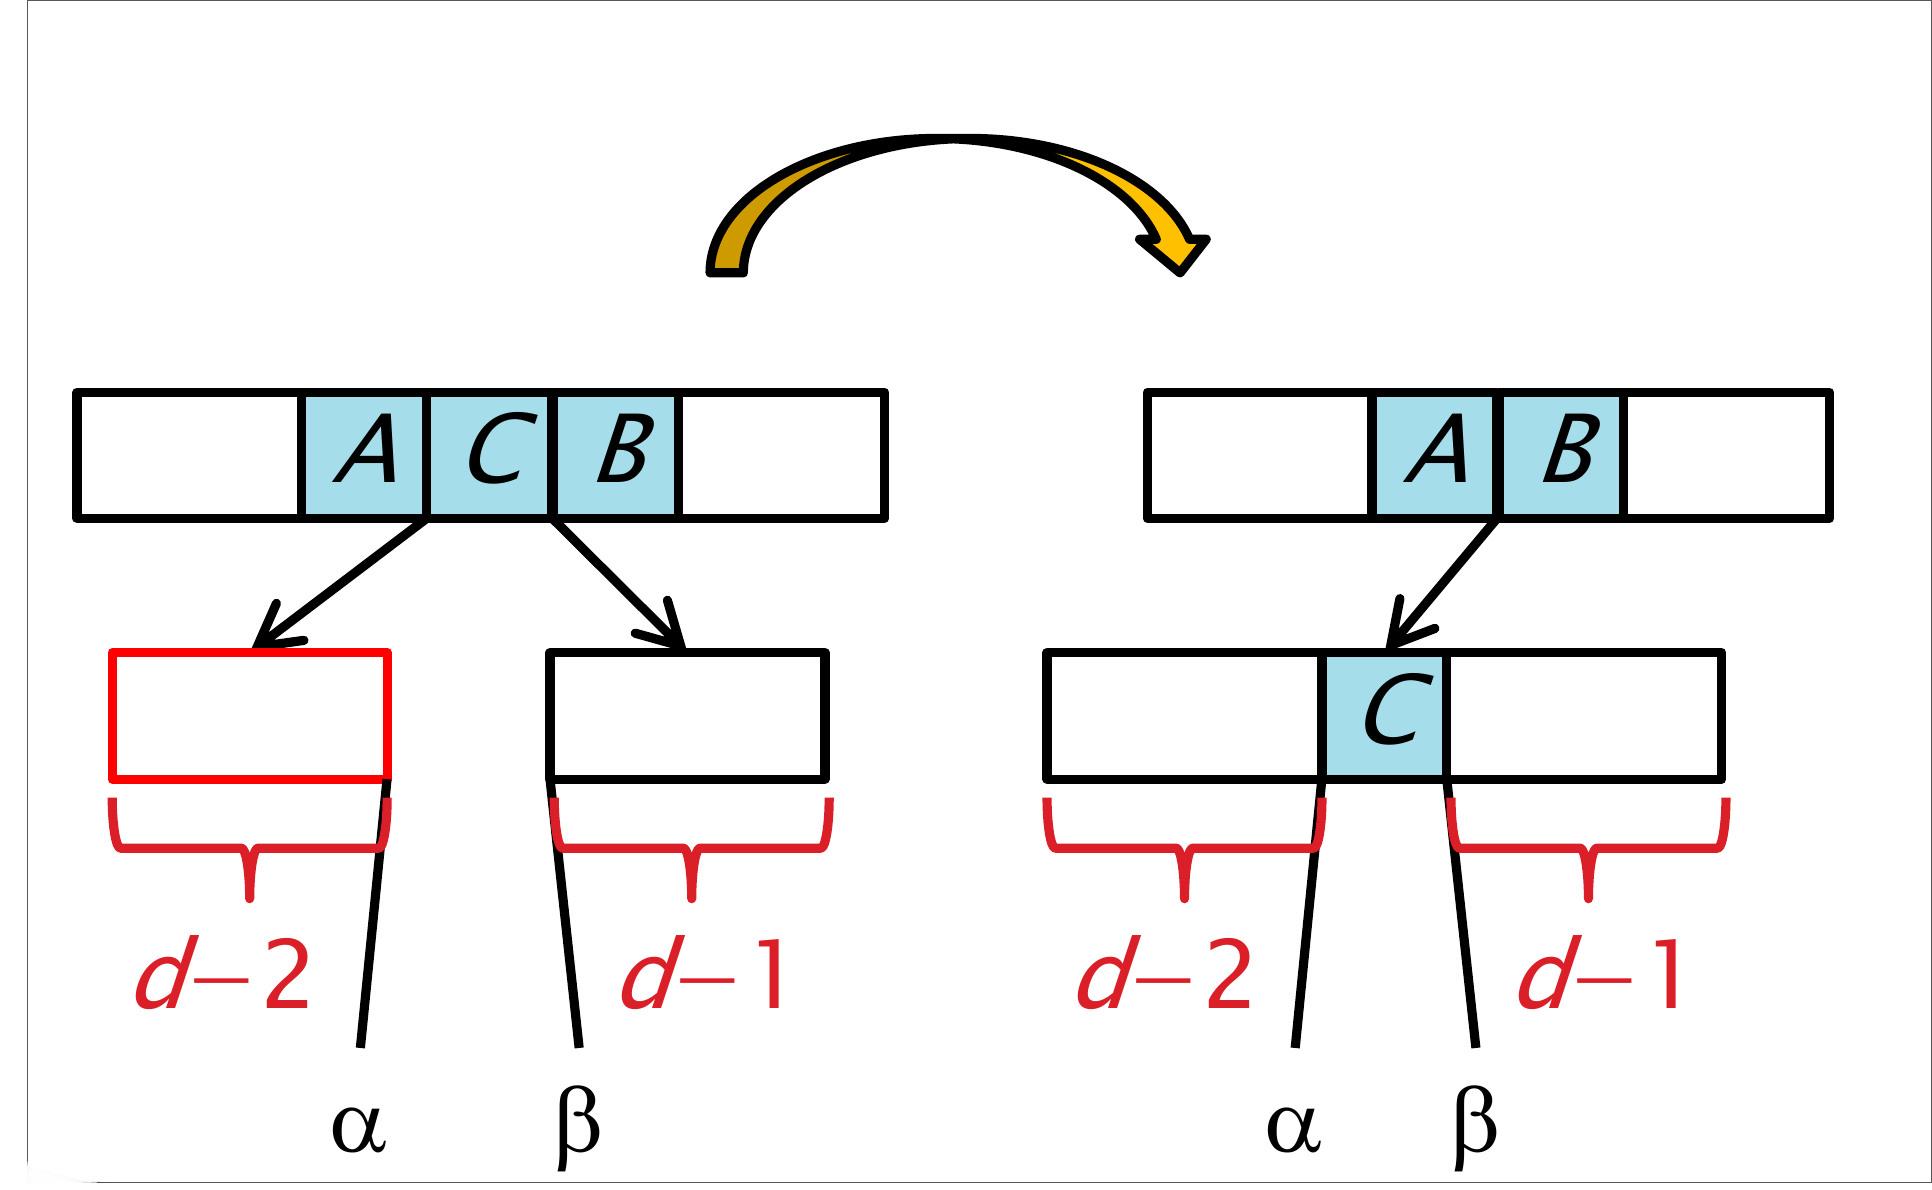
\includegraphics[width=0.45\linewidth]{images/fuse}
					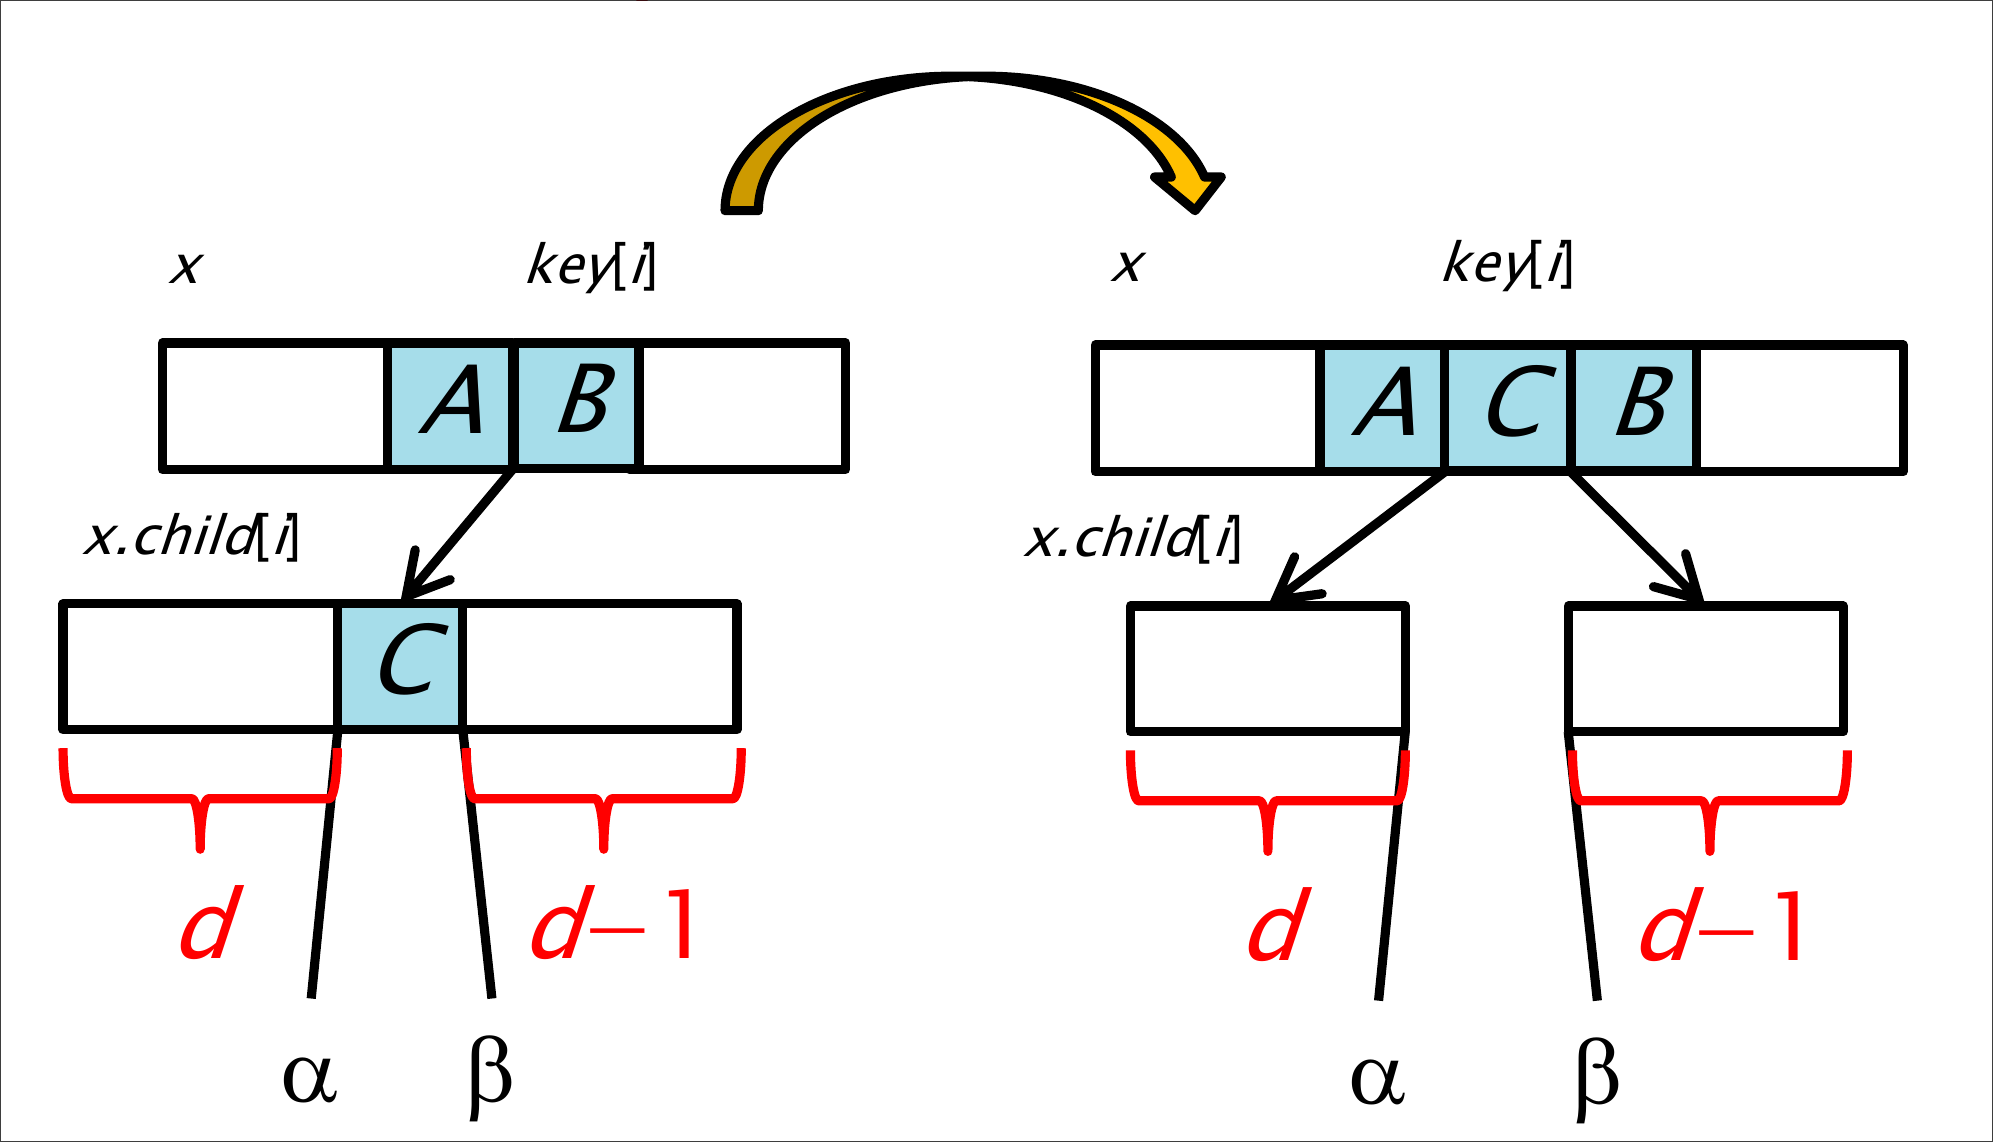
\includegraphics[width=0.485\linewidth]{images/splits} \\
					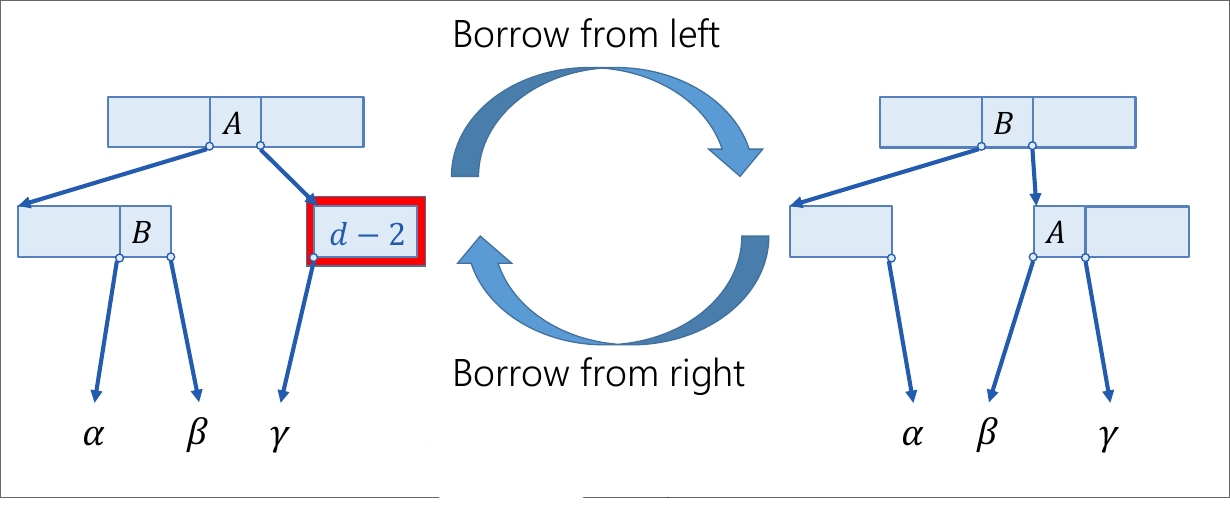
\includegraphics[width=0.55\linewidth]{images/borrow}
				\end{center}\vspace{-10pt}
				
				\quad\textbf{\textit{Insertions}}
				
					\textbf{Button-Up. }Find and insert in the appropriate leaf. If the current node is overflowing: split. If the parent is overflowing: split (etc., recursively). Requires a total of $\oc(d \log_dn)$ operations. \\
					\textbf{Top-Down. }if a node is full, we will split it on the way down while searching. \\
					\textbf{Button-Up non-leaf deletion. }replace the item by its predecessor and delete the predecessor (must be a leaf). 
				
				\quad\textbf{\textit{Deletions}}
				
					\textbf{Button-Up leaf deletion. }if the current node is underflowing, borrow and terminate and if not possible fuse and recursively check the if parent if underflowing. \\
					\textbf{Top-Down leaf deletion. }while searching, checking if the items along the way contains $d$ keys, otherwise borrow or fuse. \\
					\textbf{Top-Down non-leaf deletion. }replace the node with its predecessor, while making sure that nodes along the way contains at least $d$ keys. 
		
		\vspace{-2pt}
		\vspace{-3pt}
		\compactsection{Priority Queues}\subsectionrightaftersection
			\vspace{-4pt}
			\compactsubsection{Binary Heap}
				\begin{Definition}[binary minimum binary heap]
					an almost perfect BST (only possibly misses nodes at the last level), and satisfies the heap order: the keys at the children of $v$ are greater than they key in $v$. 
				\end{Definition}
				\lem{the height of binary heap is $\floor{\logn}$}				
				\textbf{Heap to array. }in a $d$-ary heap representation as an array (in brackets for binary, see image): 
				\vspace{-7pt}\begin{gather*}
					\textstyle \text{\rm Left}(i) = dk - (d-2) \quad (2i) \quad \text{\rm Right}(i) = dk + 1 \quad (2i + 1) \\ 
					\textstyle \text{\rm Parent}(i) = \floor{\frac{k + (d - 2)}{d}} \quad\cl{\floor{\frac{i}{2}}}
				\end{gather*}\vspace{-11pt}
				\begin{wrapfigure}{r}{0.5\linewidth}
					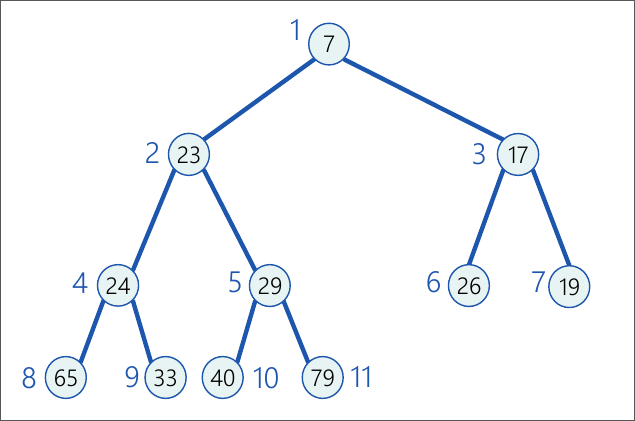
\includegraphics[width=\linewidth]{images/binaryHeapIntoArray}
				\end{wrapfigure}
				\textbf{\texttt{Heapify-Down($i$): }}if $\texttt{Parent(i)}$ is bigger, then replace $i$ with $\texttt{Parent}(i)$, and recursively continue on $\texttt{Parent(i)}$. \\
				\textbf{\texttt{Heapify-Up($i$): }} exchange with the smallest child until fixed. \\
				\textbf{\texttt{Insert}: }insert on the last place in the array, then heapify up. \\ 
				\textbf{\texttt{Delete}: }delete the required place in the array (the root) the replace it with the last one, then heapify down until fixed (in $d$-ary $\oc(d\log_dn)$). \\
				\textbf{\texttt{Dec-Key}: }decrease the key (assumes $\Delta \ge 0$) then heapify up. \\
				\textbf{\texttt{Init}: }iterate over internal nodes bottom-up, and heapify-down each one. \\
				\textbf{HeapSort: }create a min-heap from input, the do delete-min and put the deleted element at the last position of the array. Repeat $n$ times. At the we get a reversely-sorted array (using min-heaps). 
			
			\vspace{-5pt}
			\compactsubsection{Binomial Trees}
				\defi{$B_k$ is a binomial tree of degree $k$ if
				
				\hfil \begin{forest}
						[$\cdot$
							[$B_0$]
							[$B_1$]
							[$\cdots$]
							[$B_{k - 1}$]
						]
				\end{forest} ($\equiv$) \begin{forest}
					[$B_{k - 1}$
						[,no edge]
						[$B_{k - 1}$]
					]
				\end{forest}}
				\vspace{36pt}
				\theo{(1) The root of $B_k$ has $k$ children (2) $B_k$ contain $2^{k}$ nodes (3) its depth is $k$ (4) $\binom{k}{i}$ of the nodes of $B_k$ are at level $i$. }
				\begin{Definition}[Binomial Min-Heap]
					a list of heap-ordered binomial trees, at most one of each degree, and a pointer to the root with the minimal key. 
				\end{Definition}
				\begin{Remark}
					usually the trees are saved using a linked list. 
				\end{Remark}
				\lem{There are at most $\floor{\logn} + 1$ trees. }
				\textbf{\texttt{Link}: }if two binomial trees $x, y$ has the same degree, linking could be preformed in $\oc(1)$ by attaching $y$ as a child of $x$ and replacing the roots if needed. \\
				\textbf{\texttt{Insert}: }insertion could be done the same way as binary incrementing, where linking$\equiv$carrying. \\
				\textbf{\texttt{Dec-Key}: }just heapify up as before. \\
				\textbf{\texttt{Meld}: }link trees with the same degree, like binary addition. \\
				\textbf{\texttt{Del-Min}: }the children of the deleted root are a binomial heap, \texttt{Meld} them into the main tree. \\
				\textbf{Lazy Binomial Trees} adds just $B_0$-s (allows melding in $\oc(1)$), and consolidates when runs delete-min. \\
				\textbf{Consolidating} (on del-min) is the process of taking the nodes and adding them into respected bins (numbered $0 \dots \floor{\logn}$), and when two trees are in the same bin -- linking them together and moving them into the next bin. 
				\defi{$T_0$ is $\#$trees before Del-Min, $T_1$ after Del-Min, and $L$ is the total $\#$Links through consolidating. }
				\lem{$L \le T_0 + \logn$ (we have at most $\floor{\logn}$ trees exposed on Del-Min)}
				\theo{The cost of consolidating is $T_0 - 1 + \logn + L = \Theta(T_0 + \logn)$. }
				\theo{Using $\Phi = \# trees$ we get $\Dg \Phi = T_1 - T_0$ hence amort. cost of consolidating is $\oc(\logn)$. }
				\lem{incrementing a binary number has an amortized bound of $O(1)$. }
			
			\vspace{-6pt}
			\compactsubsection{Fibonazi Heaps}
				\begin{wrapfigure}{r}{0.6\linewidth}
					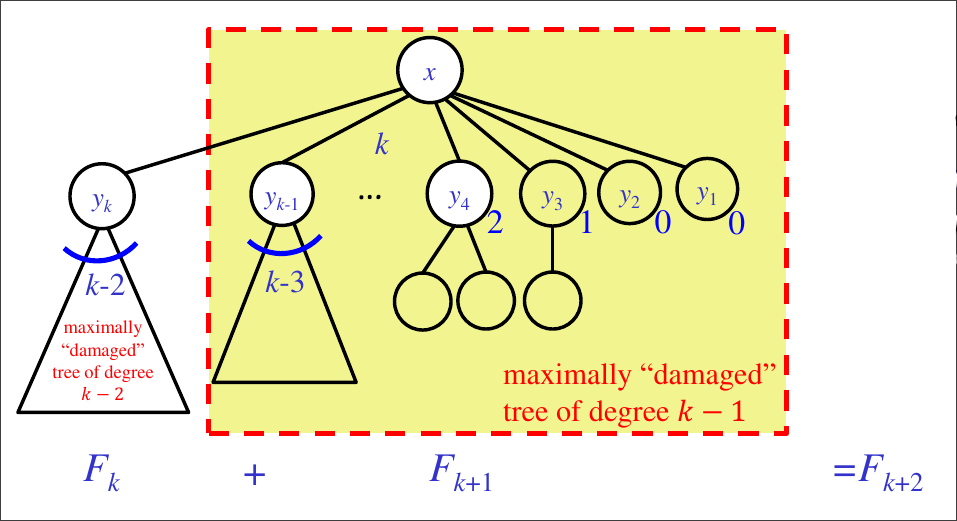
\includegraphics[width=\linewidth]{images/maxDamageFibonazi}
				\end{wrapfigure}
				\textbf{\texttt{Dec-Key}: }using cascading cuts: cut the node. Then if the parent marked as ``LOSER'' remove him too, otherwise mark it as a LOSER. Outcome: a parent with more than 2 children taken out, is taken out too. 
				\begin{Remark}
					a node in a fiboancci-heap has degree $k$ if the root has $k$ children (see image for a maximally damaged one). 
				\end{Remark}
				
				\lem{let $x$ be a node with degree $k$, and let children $y_1 \dots y_k$ be its children (in the linking order), then $y_i$'s degree is at least $i - 2$. }
				\lem{A node with deg. $k$ has at least $f_{k + 2} \ge \phi^{k}$ descendants (including) . }
				\lem{in a fib. heap all degrees are at most $\log_{\phi}n \le 1.44 \log n$}
				\theo{For a potential of $\Phi = \# \mathrm{trees} + 2\# \mathrm{marked nodes}$, we get \texttt{Dec-Key} in amort. $\oc(1)$. }
				\begin{Remark}
					actual cost of del-min is $T_0 + \logn$ and of dec-key is $+c$ ($c$ no. newly created trees). With the potential above, for dec-key we get $\Dg = 2(2 - c)$. 
				\end{Remark}
		
		\compactsection{Sorting}\subsectionrightaftersection
			\compactsubsection{Comparison-based sorting}
				\begin{Definition}[Insertion Sort]
					at iteration $i \in [n]$, by induction we assume $A[1] \cdots A[i - 1]$ is sorted, $A[i]$ ``bubble-up'' until $A[1] \cdots A[i]$ is sorted ($\oc(i)$ per iteration). 
				\end{Definition}
				\begin{Remark}
					can be optimized (in terms of exchanges, but not comparison) if $A[i]$ is saved separately. 
				\end{Remark}
				\begin{Definition}[Online sort]a sorting algorithem that doesn't have the whole input at the beginning (e.g. insertion sort)
				\end{Definition}
				\theo{insertion sort using AVL tree with insertion from the maximum, and $I > n$ inversions ($I \le \binom{2n}{n}$) takes $\oc\cl{n \log \frac{I}{n}}$. }
				\begin{Definition}[stable sort]
					 a sorting algo. the preserves order of items with the same key. 
				\end{Definition}
				\defi{a comparison-based algo. uses only two-key comparisons to decide on key position. }
				\textbf{assumption. }two keys can be compared in $\oc(1)$, and an item can be moved in $\oc(1)$. 
				\theo{the W.C. and average case of any comparison-base sorting algo. runs in $\Omega(n \logn)$}
				\lem{comparison trees are a full binary tree, and has $\ge n!$ leafs. }
				\theo{the worst/best/average case in the comparison-based model is the max/min/average depths of the leafs. }
			\compactsubsection{Other sorting algos. }
				\textbf{HeapSort: }see 5.1. \\
				\textbf{Count Sort. }For dataset $A$, assumes $\exists R \forall a \in A \le R$ constant. Counts each element $a \in A$, takes a cumulative sum $(a_i)$, then for all $a \in A$ puts $a$ in $a_i$ and decreases $a_i \gets a_i - 1$. Takes $\oc(n + R)$. Stable sort. 
				
				\textbf{Bin Sort. }similar to count sort, takes $R$ bins and throws $A$ into them, then collects them. 
				
				\textbf{Radix sort. }For a dataset $A$ sized $n$, assumes $a \in A$ contains exactly $d$ digit and each digit is bounded by $b$. Preforms count sort on the LSD $\to$ MSD. [note: relies on count sort being stable]. Takes $\oc(d(n + b))$. 
				
				\theo{Radix sort is enough to make IBM. }
				
			\compactsubsection{QuickSort}
				\begin{center}
					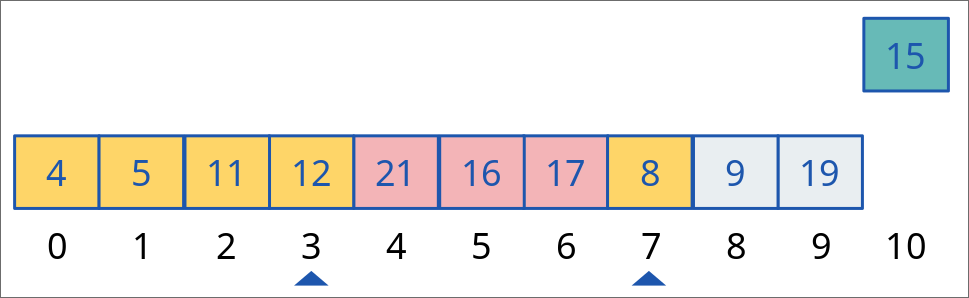
\includegraphics[width=0.51\linewidth]{images/lomuto}
					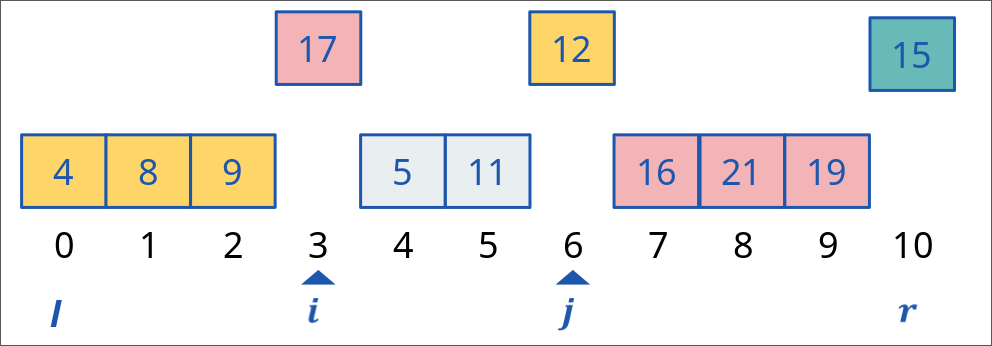
\includegraphics[width=0.45\linewidth]{images/horse}
				\end{center}

				\textbf{Lomuto's Partition. } see left image \\
				\textbf{Hoare's Partition. } see right image
				
				\begin{Remark}
					both in place $\oc(n)$, lomuto's pivot in the right place while in hoare the pivot is on the extreme right. 
				\end{Remark}
				
				\theo{W.C. of quicksort if $\binom{n}{2} = \oc(n^2)$. }
				\theo{Average case of quicksort is $2(n + 1)H_n - 4n \approx 1.39n\logn$. }
				\lem{Two keys are compared at most once by quicksort. }
				\lem{The probability that quicksort compares the $i^{\text{th}}$ smallest key with the $j^{\text{th}}$ where $i< j$ is $\frac{2}{j - i + 1}$. }
				(prove by indicator if $i, j$ compared)
		
		\compactsection{Probability}
			\begin{Definition}[Experiment]
				a case where we the result is uncertain. 
			\end{Definition}
			\begin{Definition}[Sample Space]
				the set of all the expected outcomes of a given experiment. 
			\end{Definition}
			\defi{an \color{defiColor}Event\color{black}\, is a subset of the sample space. A singleton subset called a \color{defiColor}simple event\color{black}. }
			\defi{\textit{Disjoint Events} are events $A, B$ that fulfills $A \cap B = \varnothing$. }
			\begin{Definition}[Probability Function]
				a function $P \co S \to [0, 1]$ for $S$ sample space, so that $\forall E, F \ \text{disjoint} \co P(E \cup F) = P(E) + P(F)$ and $P(S) = 1$.
			\end{Definition}
			\defi{the \color{defiColor}Conditional Probability\color{black}\, of event $E$ given the event $F$ is $P(E \mid F) := \frac{P(E \cap F)}{P(F)}$. }
			\theo{for disjoint events $(F_i)_{i = 1}^{n}$, if $\bigcup F_i = E $ then $\forall E \co P(E) = \sumni P(E \mid F_i) \cdot P(F_i)$. }
			\defi{events $E, F$ are independent if $P(E \cap F) = P(E) \cdot P(F)$ (iff $P(E \mid F) = P(E)$). }
			\begin{Definition}[Random Variable]
				a function $X \co S \to \R$. 
			\end{Definition}
			\defi{\color{defiColor}$X = x$\color{black}\, is the event on which $X(E) = x$, and its probability noted as $P(X = x)$. }
			\defi{the \color{defiColor}Expectation\color{black}\, of a random variable $X$ is $\E[x] = \sum_{x} x \cdot P(X = x)$. }\
			\theo{the expectation is linear for all constants, and additive for all random variables. }
			\defi{a random variable $I$ is called an \color{defiColor}Indicator of an event $A$\color{black}\, if $I = \begin{cases}
					1 & \text{if $A$ occurs} \\
					0 & \text{if $A^c$ occurs}
				\end{cases}$}
			\lem{$\E[I] = P(A)$. }
			\begin{Definition}[Uniform Distribution]
					of a random variable $X$ occurs when $\exists c \co \forall x \in \R \co P(X = x) = c$. 
			\end{Definition}
			\begin{Definition}[Geometric Distribution]
					satisfies $P(x = k) = (1 - p)^{k - 1}p$, hence $\E[X] = \sum_{k = 1}^{\inf} k(1 - p)^{k - 1}p = \frac{1}{p}$. 
			\end{Definition}
			\begin{Remark}
				geometric dist. is equal to having the probability of succession $p$ and for failure $p - 1$, and $P$ is a rand. var. that is equal to the number of required experiments to get to an solution. 
			\end{Remark}
			\begin{Theorem}[The Tail Formula]\!\!\!
				\hfil $\sum_{i = 0}^{m}i \cdot P[X \!=\! i] = \sum_{i = 1}^{m} \!P(x \ge i)$
			\end{Theorem}
			\begin{Theorem}[Markov's Inequality]
				\hfil $P[X \le 2\E[X]] \ge 0.5$
			\end{Theorem}
		
		\compactsection{Selection}
			\defi{given $n$ numbers, \texttt{Select($n$)} is defined to return the k$^{\text{th}}$ smallest key. }
			\begin{wrapfigure}{r}{0.4\linewidth}
				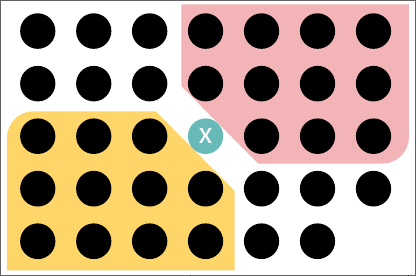
\includegraphics[width=\linewidth]{images/MedofMed}
				\vspace{-10pt}
			\end{wrapfigure}
			\textbf{E.g.} (width$=\floor{\frac{1}{2}\floor{\frac{n}{5}}}$, height$=3$, total$\ge3 \cdot \frac{n}{10} - 1 - 3$)
			This equals for the item in position $k$, assuming the array was sorted. 
			\begin{Definition}[Dynamic settings]
					assumes one-time building cost (e.g. \texttt{Tree-Select}). 
			\end{Definition}
			\begin{Definition}[Static settings]
				not a dynamic setting
			\end{Definition}
			\theo{Using min-heap + supporting heap the selection problem is solvable is $\oc(n + k \log k)$. }
			\theo{The expected number of items removed during each quickselect run is $\E[\#\text{\rm removed}] = \frac{k}{2}\cdot\frac{k}{n} + \frac{n - k}{2}\cdot\frac{n - k}{n} \underset{\forall k}{\ge} \frac{n}{4}$. }
			\theo{The expected runtime of quickselect is $\oc(n)$. }
			\theo{MedofMed cost is W.C. $\oc(n)$. }
			
		
		\compactsection{Hashing}\subsectionrightaftersection
			\textbf{Direct Addressing. }Create a bit vector with the universe size. e.g. \texttt{Insert($D, x$)} iff \texttt{D[$x$.$key$] $\gets$ $x$} etc. 
			\compactsubsection{Chaining}
				\lem{There are $|m|^{|U|}$ hashes in $h \in U \to [m]$, hence takes $|U|\log m$ to store. }
				\textbf{Chaining. }each cell points to a linked list of items. 
				\begin{Definition}[load factor]
					$\ag := \frac{n}{m}$ where $n$ is the universe, and $m$ is the table size. 
				\end{Definition}
				\lem{the probability of a random two specific insertions colliding is geometric. }
				\theo{the expected number of values in each cell is $\ag$. }
				\theo{when $n = \Theta(m)$, with probability $\ge 1 - \frac{1}{n}$, each cell contains at most $\oc\cl{\frac{\logn}{\logn\logn}}$ elements. }
				\theo{Assuming the keys are distributed ideally (uniformly and independently), and assuming $n$ keys were previously inserted, the expected complexity during search is $\ag + 1$ for unsuccessful and $\frac{\ag}{2} + 1$ for a successful search. }
			
			\compactsubsection{Open Addressing}
				\textbf{Open Addressing. }\set $h \co U \times [m] \to [m]$ be a hash function, we'll insert the key $k$ in the first free position in the probing sequence. 
				
				\begin{Remark}
					make sure to use special marking (not null) for deleted items.  
				\end{Remark}
				
				\theo{Under ideal conditions (means $\forall k \in [n] \co P\cl{(h(k, i)_{i = 0}^{m - 1}) = \frac{1}{m}}$), the expected time for unsuccessful search is $\frac{1}{1 - \ag}$ and for successful search $\frac{1}{\ag} \ln \frac{1}{1 - \ag}$. } 
				
				\theo{under linear probing, unsuccessful search takes $\frac{1}{2}\cl{1 + \cl{\frac{1}{1 - \ag}}^2}$ and successful search $\frac{1}{2}\cl{1 + \frac{1}{1 - \ag}}$. }
				\begin{Remark}
					under linear probing, we can delete by recursively checking if item $j$ can me moved to deleted cell $i$ for all $h'(T[j]) \in [j + 1, i]$. 
				\end{Remark}
				
				\textbf{Probing Sequence: }$h(k, 0) \dots h(k, m - 1)$
				
				\begin{Definition}[Linear Probing]
				 	a hash func $h(k, i) := (h'(k) + i) \bmod m$ (less cache misses + easy to calculate). 
				\end{Definition}
				\begin{Definition}[Quadratic Probing]
					a hash func $h(k, i) := (h'(k) + ic_1 + c_2i^2) \bmod m$. 
				\end{Definition}
				\begin{Definition}[Double Probing]
					a hash func $h(k, i) := (h'(k) + ih''(k)) \bmod m$. 
				\end{Definition}
			
			\compactsubsection{Hash Families}
				\defi{$\sof{Col}$ is the number of collision for a given $h$ hash. }
				\defi{hash family is \color{defiColor}Universal\color{black}\, if $\forall k_1 \neq k_2 \in U \co P_{h \in H}(h(k_1) = h(k_2)) \le \frac{1}{m}$. }
				\theo{For all $p$ prime, $h_{a, b} \co [p] \to [m]$ defined as $h_{a, b}(x) = ((ax + b) \bmod p)\bmod m$, and $H_{p, m} := \{h_{a, b} \mid a \in [1, p), b \in [0, p)\}$ is a universal hash family. }
				\theo{for each $p$ prime, \set $x_1 \neq x_2 \in [p]$. Then $\forall y_1 \neq y_2 \in [p]\,\, \exists ! a, b \in [p], a \neq 0 \co y_1 \equiv_p ax_1 + b \land y_2 \equiv_p ax_2 + b$. }
				\theo{for a table $m = 2^{k}$ so $h_a \co U = [2^{w}] \to [2^{k}]$ where $w$ is computer word size, $h_a$ defined as $\floor{\frac{ax \mod 2^{w}}{2^{w - k}}}$, and $H$ is almost universal. }
				\defi{if $\forall k_1 \neq k_2 \in U \co P_{h \in H}(h(k_1) = h(k_2)) \le \frac{2}{m}$ then $U$ is called \color{defiColor}almost universal\color{black}. }
				\theo{using universal hash family, $\E[\text{collisions}] \le \frac{\binom{n}{2}}{m}$. }
				\theo{If $m = n$, then $P(|Col| < n) \ge \frac{1}{2}$}
				\theo{If $m = n^2$, then $P(|Col| < 1) \ge \frac{1}{2}$}
				\begin{Remark}
					Theorems 40, 41 are derived from theorem 39 using Markov's inequality (see 7.0)
				\end{Remark}
		
		
			\compactsubsection{Perfect Hashing}
				\begin{wrapfigure}{r}{0.6\linewidth}
					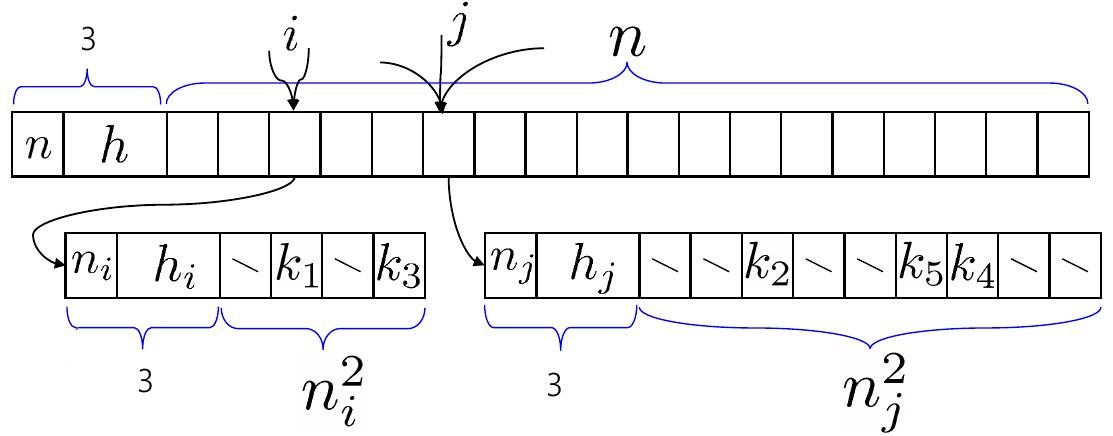
\includegraphics[width=\linewidth]{images/perfectHash}
				\end{wrapfigure}
				\textbf{\texttt{Init}: }choose random $h \in H_{p, n}$ (modular), compute the number of collision, until there are $< n$ collisions (expected $2$ attempts). Then for each cell $i \in [n]$ let $n_i := \sof{h\op[\{i\}]}$, if $n_i > 1$ choose a random $h_i \in H_{p, n_i^2}$ until there are no collisions. \\
				\textbf{Total size }$=3 + n + 3n + \sum_i n_i^2 = 4n + 3 + \sum(2\binom{n_i}{2} + n_i)$ and since $|col| = \sum_i \binom{n_i}{2}$ we get a total of $\le 7n + 3$. 
				
		
		\compactsection{Other}
			\textbf{Reduction. }reduction (in our case) is the process of showing the a problem is at least as hard as another problem. \\
			\textbf{Information Bound. }a bound derive by an argument that the algo. has to read a specified amount of the input, in order to get a decision. Notice that in comparison, reading isn't counted. 
			\vspace{-9pt}\begin{align*}
				\textstyle \sum_{i = 1}^{k}\binom{k}{i} = 2^{k} \quad&\quad\quad \textstyle \binom{k}{i} = \binom{k - 1}{i} + \binom{k - 1}{i - 1} \\ 
				\textstyle a_i = a_1 + (n - 1)d \implies \sumni a_i  &= \textstyle \frac{n(a_1 + a_n)}{2} \\
				\textstyle a_i = a_1 q^{n - 1} \implies \sumni a_i   &=  \textstyle \frac{a_1(q^{n} - 1)}{q - 1}
			\end{align*}\vspace{-15pt}
			\theo{merging $k$ sorted arrays with the total of $n$ items can be done in $\oc(n \floor{\log k})$}
			\theo{Fibonacci closed form. $\textstyle F_n = \frac{\phi^{n} - (\bar \phi)^{n}}{\sqrt 5}$ where $\textstyle \Phi = \frac{1 + \sqrt 5}{2}$}
			\begin{wrapfigure}{r}{0.5\linewidth}
				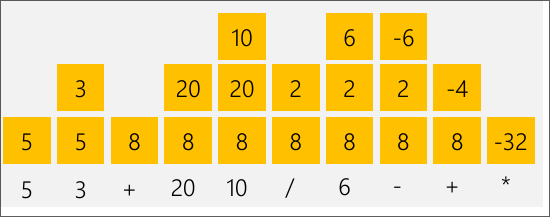
\includegraphics[width=\linewidth]{images/postfix}
			\end{wrapfigure}
			\textbf{Postfix syntax algo. }parse mathematical expressions. For each element $e$ from left to right: (1) if $e$ is operand then push $e$ (2) if $e$ binary operator, pop 2 elements $x, y$ then push $e(x, y)$, and if $e$ unary operator pop 1 element $x$ and push $e(x)$ (see image). 
			\textbf{Jensen's inequality. }$\textstyle f(\frac{x_1 + x_2}{2}) \le \frac{f(x_1) + f(x_2)}{2}$ if $f$ convex. 
		
			\compactsubsection{Array Doubling}
				\textbf{Potential for doubling by $(1 + \ag)$. }$\Phi := \begin{cases}
					\frac{1 + \ag}{\ag} n - \frac{M}{\ag} & \!n > \frac{M}{\ag + 1} \\
					0 & \!\other
				\end{cases}$
				\!\!yields to amort. bound $\oc\cl{\frac{1 + \ag}{\ag} + 1}$ \\
				\begin{wrapfigure}{r}{0.5\linewidth}
					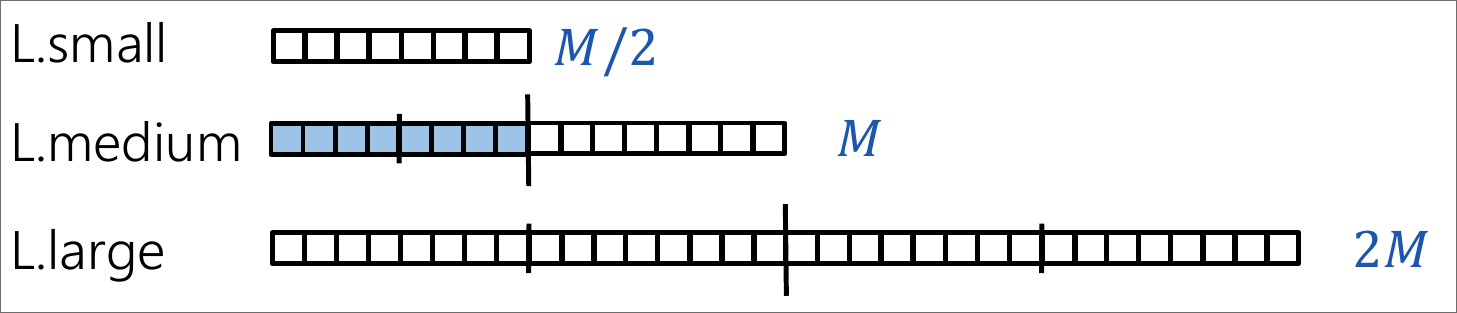
\includegraphics[width=\linewidth]{images/deAmoritzedArray}
					\vspace{-10pt}
				\end{wrapfigure}
				\textbf{Potential for array doubling} (including amort deletion: changing the size back when $n = \frac{M}{4}$)\textbf{. }
				
				\vspace{-5pt}
				\hfil $\Phi = \begin{cases}
					2n - M & \text{if}\, n \ge \frac{M}{2} \\
					\frac{M}{2} - n & \text{if}\, n < \frac{M}{2}
				\end{cases}$
				
				\textbf{De-Amortized array doubling. }see image \\
		% Additional notes may go here
		
	\end{multicols}
	
	\vspace{-10pt}
	\compactsection{Complexity Tables}
	\vspace{-15pt}
	\begin{multicols}{2}
		{\regFont\hfil \textbf{Lists}}\tableFont
		
		{\hfil $\set \midText := \min\{i, n - i\} + 1$}
		\begin{center}
			\begin{tabular}{c|c|c|c|c|c|c}
				& \texttt{Ins/Del-Last} & \texttt{Ins/Del-First} & \texttt{Insert($i$)} & \texttt{Retrieve($i$)} &
				\texttt{Concat($n_1, n_2$)} & \texttt{Split($i$)} \\
				\hline
				\textbf{Arrays} & $\oc(1)$ & $\oc(n + i)$ & $\oc(n - i + 1)$ & $\oc(1)$  & $\oc(n_2 + 1)$ & $\oc(n - i + 1)$ \\
				\textbf{Circular Arr.} & $\oc(1)$ & $\oc(1)$ & $\oc(\midText)$ & $\oc(1)$ & $\oc(\min\{n_1, n_2\})$ & $\oc(\midText)$ \\ 
				\textbf{D-Linked} & $\oc(1)$ & $\oc(1)$ & $\oc(\midText)$ & $\oc(\midText)$ & $\oc(1)$ & $\oc(\midText)$ \\ 
				\textbf{AVL List} & $\oc(\logn)$ & $\oc(\logn)$ & $\oc(\logn)$ &$\oc(\log i + 1)$ & $\oc(\log(n_1 + n_2))$ & $\oc(\logn)$
			\end{tabular}
		\end{center}
		(in a lazy doubly-linked list, amortized del./ins. $\oc(1)$ and ret. $\oc(i + 1)$)
		% Additional notes may go here
		
		\columnbreak
		{\regFont\hfil \textbf{Priority Queues}}\tableFont 
		\begin{center}\begin{tabular}{c|c|c|c|c|c|c|c}
				& \textbf{\texttt{Insert}} & \textbf{\texttt{Minimum}} & \textbf{\texttt{Delete-Min}} & \textbf{\texttt{Dec.-Key}} & \textbf{\texttt{Delete}({\rm pointer})} & \textbf{\texttt{Meld}} & \textbf{\texttt{Init}} \\
				\hline
				\textbf{AVL tree} & $\oc(\logn) $ & $\oc(1)$ & $\oc(\logn)$ & $\oc(\logn)$ & $\oc(\logn)$ & $\oc(n)$ & $\oc(n \logn)$ \\
				\textbf{Binary Heap} & $\oc(\logn)$ & $\oc(1)$ & $\oc(\logn)$ & $\oc(\logn)$ & $\oc(\logn)$ & $\oc(n)$ & $\oc(n)$ \\
				\textbf{W.C Binomial Heap} & $\oc(\logn)^{(*)}$ & $\oc(1)$ & $\oc(\logn)$ & $\oc(\logn)$ & $\oc(\logn)$ & $\oc(\logn)$ & $\oc(n)$ \\
				$\overset{\text{\tableFont \textbf{Lazy Amort./WC}}}{\text{\tableFont \textbf{Binomial Stack}}}$
				& $\oc(1)_{W.C.}$ & $ \oc(1)_{W.C.} $ & \tline{$\oc(\logn)$}{$\oc(n)_{W.C.}$} & $\oc(\logn)_{W.C.}$ & \tline{$\oc(\logn)$}{$\oc(n)_{W.C.}$} & $\oc(1)_{W.C.}$ & $\oc(n)_{W.C.}$ \\
				\tline{\textbf{Amort./WC}}{\textbf{Fib. Heap: }}& $\oc(1)_{W.C.}$ & $ \oc(1)_{W.C.} $ & \tline{$\oc(\logn)$}{$\oc(n)_{W.C.}$} & $\oc(1)_{W.C.}$ & \tline{$\oc(\logn)$}{$\oc(n)_{W.C.}$} & \tline{$\oc(1)$}{$\oc(n)_{W.C.}$} & $\oc(n)_{W.C.}$ \\
			\end{tabular}\end{center}
			$^{(*)}$amortized $\oc(1)$ for a sequence of operations from the same type. 
	\end{multicols}
	% Additional notes may go here
	\vfil
	\textbf{I may have mistakes and correctness is not guaranteed $\sim$ Shahar Perets $\sim$ Data Structures 2025B $\sim$ Shit Cheat Sheet}
	
%	\vspace{-4.5em}\vspace{-8em}
	
	
\end{document}